
\section{Rückblick}

\begin{frame}
  {Wortklassen: Grundlagen}
  \pause
  \begin{itemize}[<+->]
    \item Wortklassen als \alert{Grundausstattung der Grammatik}
    \item Vehikel für klassenbezogene Generalisierungen
    \item Bedeutung? --- nicht alle Wörter
      \Zeile
    \item Wortform\slash syntaktisches Wort:
      \begin{itemize}[<+->]
        \item konkrete Form \alert{im syntaktischen Kontext}
        \item voll spezifiziert (Merkmale, Werte)
      \end{itemize}
      \Zeile
    \item Wort\slash lexikalisches Wort:
      \begin{itemize}[<+->]
        \item abstrakte Form \alert{im Lexikon}
        \item evtl.\ unterspezifiziert
      \end{itemize}
      \Zeile
    \item "`Schulwortarten"': \alert{unzureichend operationalisiert}
  \end{itemize}
\end{frame}

\section{Überblick}

\begin{frame}
  {Morphologie: Flexion und Wortbildung}
  \pause
  \begin{itemize}[<+->]
    \item \alert{Formveränderungen} und \alert{Merkmalsänderungen}
      \begin{itemize}[<+->]
        \item Veränderungen von Werten
        \item Veränderungen von Merkmalsaustattungen
      \end{itemize}
      \Halbzeile
    \item Morphe (= Wortbestandteile) und ihre Funktionen
    \item Morphe: alle Stämme und alle nicht-lexikalischen Morphe
      \Halbzeile
    \item statische und volatile Merkmale
    \item Wortbildung vs.\ Flexion, definiert anhand von Merkmalen
  \end{itemize}
\end{frame}

\begin{frame}
  {Morphologie und Bildungssprache\slash Normsprache}
  \pause
  \begin{itemize}[<+->]
    \item Flexion und zugehörige Funktionskategorien
      \begin{itemize}[<+->]
        \item normsprachlich überwiegend \alert{klar definiert}
        \item vorliterate perfekte Beherrschung nicht voraussetzbar (z.\,B.\ Konjunktiv)
          \Halbzeile
        \item erhebliche Abweichungen in \alert{Dialekten}, \alert{Soziolekten} und \alert{Kiezsprachen}
          \Halbzeile
        \item \textit{Et rēchnet aufe Terasse.} (Pott)
        \item Aber wie funktioniert das eigentlich genau?
          \Halbzeile
        \item \textit{Ich las schon einmal Rilke.} (rhfr. Hyperkorrektur)
        \item Im Odenwald gibt es kein Präteritum, wird in der Schule gelernt.
      \end{itemize}
     \Halbzeile 
    \item Wortbildung
      \begin{itemize}[<+->]
        \item wichtiger Kern der Bildungssprache (besonders Komposition)
          \Halbzeile
        \item \textit{Das ist wegen der Spannendheit.} (Kind, 7--8 Jahre, ca. 1992)
        \item \textit{Die Vase ist vollansichtlich reliefiert.} (Heide Rezepa-Zabel, 2018)
      \end{itemize}
  \end{itemize}
\end{frame}

\begin{frame}
  {Morphosyntax in der Schule}
  \pause
  Wozu ist so ein Unterricht gut?
  \pause
  \begin{center}
    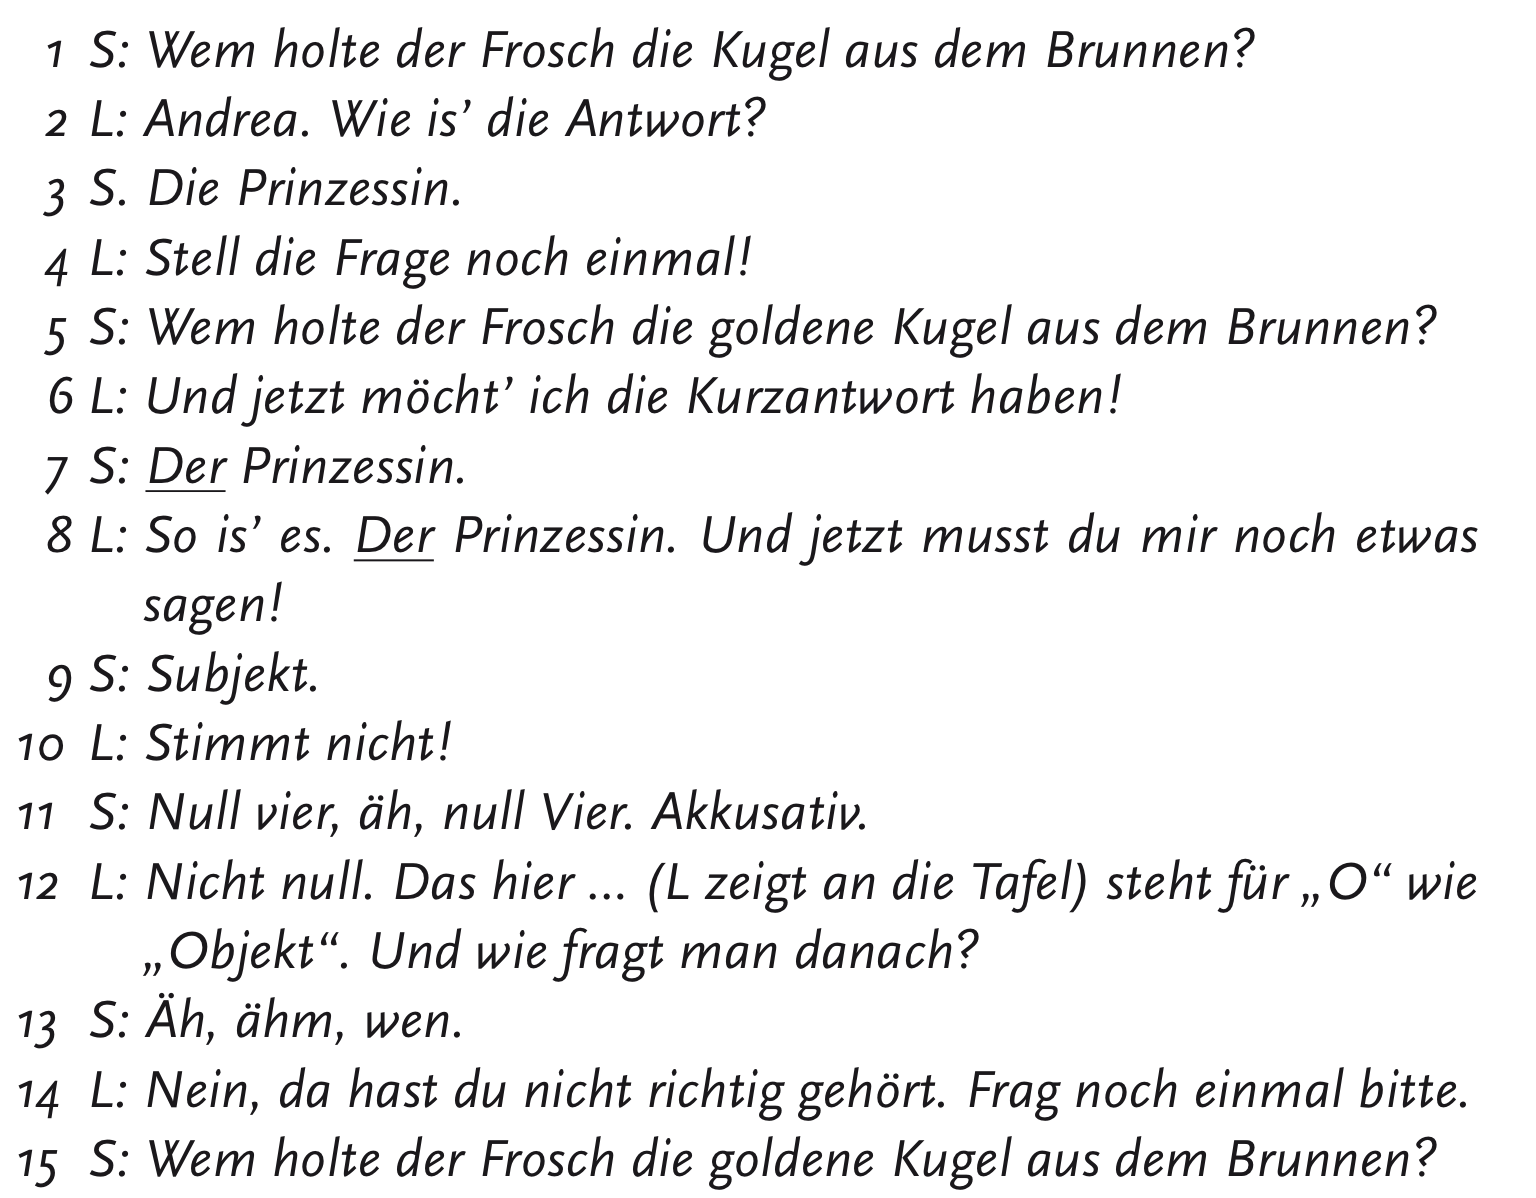
\includegraphics[width=0.6\textwidth]{graphics/kasusschule1}
  \end{center}
  \tiny \citet[36--37]{Gramzowemden2002}, zitiert nach \citet[257--258]{Bredel2013}
\end{frame}

\begin{frame}
  {Morphosyntax in der Schule}
  Wozu ist so ein Unterricht gut?
  \begin{center}
    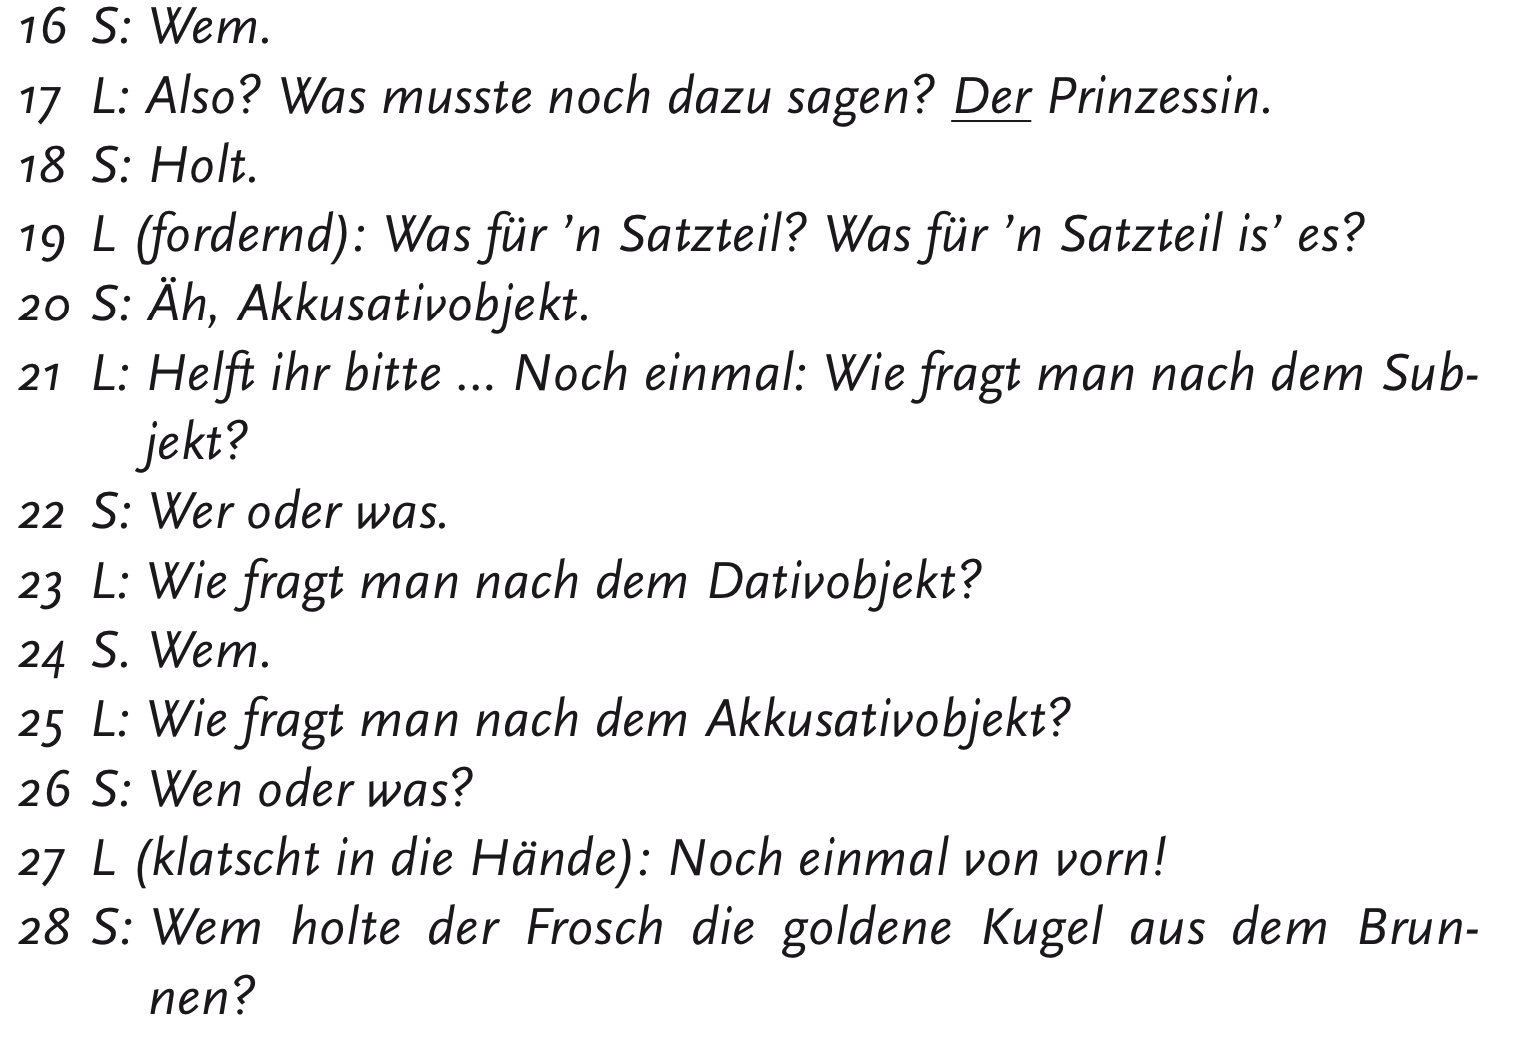
\includegraphics[width=0.6\textwidth]{graphics/kasusschule2}
  \end{center}
  \tiny \citet[36--37]{Gramzowemden2002}, zitiert nach \citet[257--258]{Bredel2013}
\end{frame}

\begin{frame}
  {Morphosyntax in der Schule}
  Wozu ist so ein Unterricht gut?
  \begin{center}
    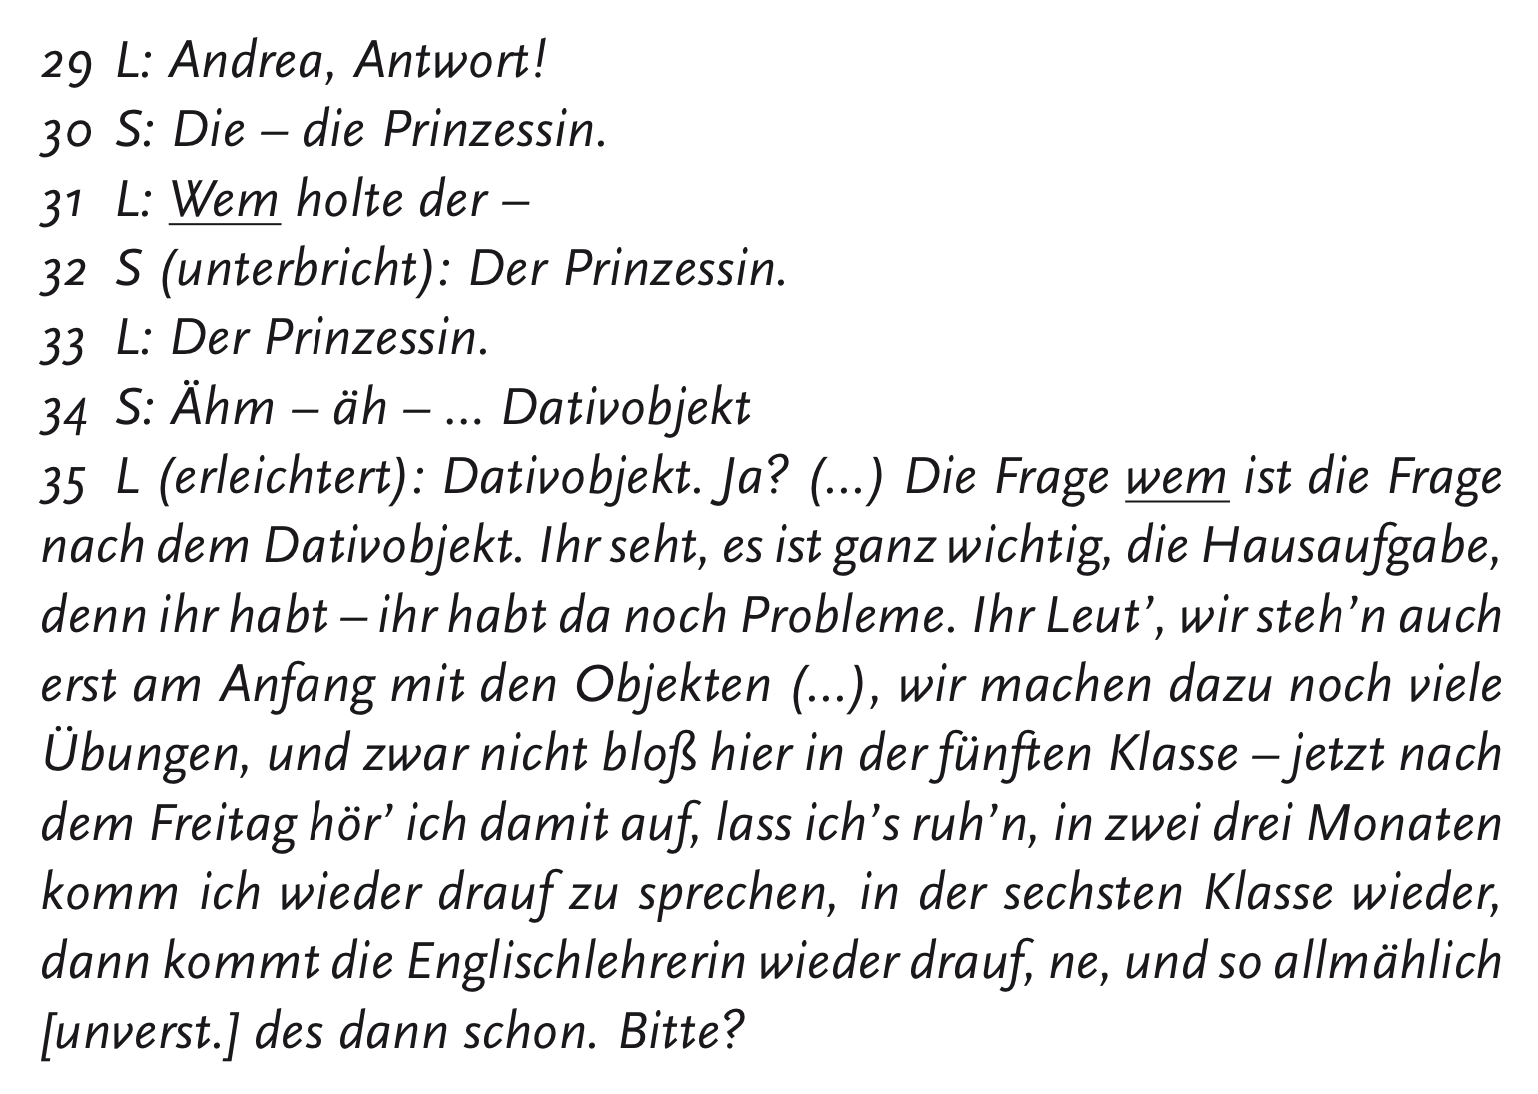
\includegraphics[width=0.6\textwidth]{graphics/kasusschule3}
  \end{center}
  \tiny \citet[36--37]{Gramzowemden2002}, zitiert nach \citet[257--258]{Bredel2013}
\end{frame}

\section{Stämme und Affixe}

\begin{frame}
  {Form und Funktion: Flexion}
  \pause
  \begin{exe}
    \ex
    \begin{xlist}
      \ex \alert{Den Präsidenten} begrüßte \alert{der Dekan} äußerst respektlos.
      \pause
      \ex \alert{Der Dekan} begrüßte \alert{den Präsidenten} äußerst respektlos.
    \end{xlist}
    \pause
    \ex
    \begin{xlist}
      \ex \alert{Die Präsidentin} begrüßte \alert{die Dekanin} äußerst respektlos.
      \pause
      \ex \alert{Die Dekanin} begrüßte \alert{die Präsidentin} äußerst respektlos.
    \end{xlist}
  \end{exe}
  \pause
  \Zeile
  Formveränderungen lexikalischer Wörter \alert{schränken ihre möglichen grammatischen Funktionen und Relationen im Satz ein}\dots\\
  \pause
  \Halbzeile
  \dots und sie haben semantische und systemexterne Folgen.

\end{frame}

\begin{frame}
  {Form und Funktion: Wortbildung}
  \pause
  \begin{exe}
    \ex grün\alert{lich}, röt\alert{lich}, gelb\alert{lich}
    \pause
    \ex Neu\alert{igkeit}, Blöd\alert{heit}, Tauch\alert{er}, Heb\alert{ung}
    \pause
    \ex Fenster\alert{rahmen}, Tücher\alert{spender}, Glas\alert{korken}, Unter\alert{schrank}
  \end{exe}
  \pause
  \Zeile
  Formveränderungen von einem zu einem anderen lexikalischen Wort führen zu Bedeutungs- und kategorialen Veränderungen.
\end{frame}

\begin{frame}
  {Markierungsfunktionen von Morphen I}
  \pause
  \begin{exe}
    \ex
    \begin{xlist}
      \ex{(der) \alert<4>{Berg}}
      \ex{(den) \alert<4>{Berg}}
      \ex{(dem) \alert<4>{Berg}}
      \ex{(des) \alert<5>{Berg}\rot<5>{-es}}
      \ex{(die) \alert<6>{Berg}\rot<6>{-e}}
      \ex{(der) \alert<6>{Berg}\rot<6>{-e}}
    \end{xlist}
    \pause
    \ex
    \begin{xlist}
      \ex{(der) \alert<8>{Mensch}}
      \ex{(den) \alert<9>{Mensch}\rot<9>{-en}}
      \ex{(dem) \alert<9>{Mensch}\rot<9>{-en}}
      \ex{(des) \alert<9>{Mensch}\rot<9>{-en}}
      \ex{(die) \alert<9>{Mensch}\rot<9>{-en}}
      \ex{(der) \alert<9>{Mensch}\rot<9>{-en}}
    \end{xlist}
  \end{exe}
\end{frame}

\begin{frame}
  {Markierungsfunktionen von Morphen II}
  \pause
  \begin{exe}
    \ex
    \begin{xlist}
      \ex{(ich) \alert<3>{kauf}\rot<3>{-e}}
      \ex{(du) \alert<4>{kauf}\rot<4>{-st}}
      \ex{(wir) \alert<5>{kauf}\rot<5>{-en}}
      \ex{(sie) \alert<5>{kauf}\rot<5>{-en}}
    \end{xlist}
  \end{exe}
\end{frame}

\begin{frame}
  {Morphe und Markierungsfunktionen}
  \pause
  \begin{itemize}[<+->]
    \item Formveränderungen:
      \begin{itemize}[<+->]
        \item oft nicht \alert{eine} Funktion
        \item \rot{Einschränkung} der möglichen Funktionen
      \end{itemize}
   \Halbzeile 
    \item \alert{Markierungsfunktion}: eine \alert{Reduktion}\\
      der möglichen Merkmale oder Werte einer Wortform
    \item zum Beispiel \textit{-en} bei schw.\ Maskulina: \rot{nicht} Nominativ Singular
    \item oder \textit{-en} bei Verben im Präsens: Plural und nicht adressatbezogen
      \Halbzeile
    \item \alert{Morphe = alle segmentalen Einheiten mit Markierungsfunktion}
    \item konkret: \alert{Stämme} und \alert{Affixe}
  \end{itemize}
\end{frame}

\begin{frame}
  {Stämme I}
  \pause
  \begin{exe}
    \ex
    \begin{xlist}
      \ex{(ich) \alert<5->{kauf}-e\\
        (du) \alert<5->{kauf}-st\\
        (ihr) \alert<5->{kauf}-t }
        \pause
        \ex{(ich) \alert<6->{kauf}-te\\
        (du) \alert<6->{kauf}-test\\
        (ihr) \alert<6->{kauf}-tet}
        \pause
        \ex{(ich habe) ge-\alert<7->{kauf}-t\\
        (du hast) ge-\alert<7->{kauf}-t\\
        (ihr habt) ge-\alert<7->{kauf}-t}
    \end{xlist}
  \end{exe}
\end{frame}

\begin{frame}
  {Stämme II}
  \begin{exe}
    \ex
    \begin{xlist}
      \ex{(ich) \alert<4->{nehm}-e\\
        (du) \rot<5->{nimm}-st\\
          (es) \rot<5->{nimm}-t\\
          (ihr) \alert<4->{nehm}-t}
        \pause
        \ex{(ich) \orongsch<6->{nahm}\\
        (du) \orongsch<6->{nahm}-st\\
          (ihr) \orongsch<6->{nahm}-t}
        \pause
        \ex{(ich habe) ge-\gruen<7->{nomm}-en\\
        (du hast) ge-\gruen<7->{nomm}-en\\
        (ihr habt) ge-\gruen<7->{nomm}-en}
    \end{xlist}
  \end{exe}
  \pause
  \pause
  \pause
  \pause
  \pause
  Der \alert{Stamm} kann nicht "`der unveränderliche Wortbestandteil"'\\
  eines lexikalischen Wortes (in einem Paradigma) sein.\\
  \Zeile
  \pause
  \alert{\dots aber der mit der Bedeutung, also der lexikalischen Markierungsfunktion}!
\end{frame}

\begin{frame}
  {Affixe}
  \pause
  \begin{exe}
    \ex
    \begin{xlist}
      \ex (ich) nehm\alert<6->{-e}
      \pause
      \ex (des) Berg\alert<7->{-es}
      \pause
      \ex Schön\alert<8->{-heit}
      \pause
      \ex \alert<9->{Un-}ding
    \end{xlist}
  \end{exe}
  \Zeile
  \pause
  \pause
  \pause
  \pause
  \pause
  \begin{itemize}[<+->]
    \item \alert{keine lexikalische Markierungsfunktion} (= keine eigene Bedeutung)
    \item \alert{nicht wortfähig} = nicht ohne Stamm verwendbar
  \end{itemize}
\end{frame}



\section{Merkmale in Flexion und Wortbildung}

\begin{frame}
  {Statische und volatile Merkmale}
  \pause
  \begin{itemize}[<+->]
    \item Eigenschaften: "`Rotsein"' (Erdbeere), "`325m hoch"' (Eiffelturm) usw.
    \item Merkmale: \alert{\textsc{Farbe}}, \alert{\textsc{Länge}} usw.
    \item Werte:
      \begin{itemize}[<+->]
        \item \alert{\textsc{Farbe}}: \rot{\textit{rot}}, \rot{\textit{grau}}, \ldots
        \item \alert{\textsc{Länge}}: \rot{\textit{3cm}}, \rot{\textit{325m}}, \ldots
      \end{itemize}
  \end{itemize}
  \pause
  \Halbzeile 
  \begin{exe}
    \ex
    \begin{xlist}
      \ex{Haus = [\textsc{Bed}: \gruen<12->{\textbf{\textit{haus}}}, \textsc{Klasse}: \gruen<12->{\textbf{\textit{subst}}}, \textsc{Gen}: \gruen<12->{\textbf{\textit{neut}}}, \textsc{Kas}: \orongsch<13->{\textit{nom}}, \textsc{Num}: \orongsch<13->{\textit{sg}}]}
      \pause
      \ex{Haus-es = [\textsc{Bed}: \gruen<12->{\textbf{\textit{haus}}}, \textsc{Klasse}: \gruen<12->{\textbf{\textit{subst}}}, \textsc{Gen}: \gruen<12->{\textbf{\textit{neut}}}, \textsc{Kas}: \orongsch<13->{\textit{gen}}, \textsc{Num}: \orongsch<13->{\textit{sg}}]}
      \pause
      \ex{Häus-er = [\textsc{Bed}: \gruen<12->{\textbf{\textit{haus}}}, \textsc{Klasse}: \gruen<12->{\textbf{\textit{subst}}}, \textsc{Gen}: \gruen<12->{\textbf{\textit{neut}}}, \textsc{Kas}: \orongsch<13->{\textit{nom}}, \textsc{Num}: \orongsch<13->{\textit{pl}}]}
    \end{xlist}
  \end{exe}
  \Halbzeile
  \pause
  \begin{itemize}[<+->]
    \item bei einem lexikalischen Wort:
      \begin{itemize}
        \item \gruen{statische Merkmale} wertestabil
        \item \orongsch{volatile Merkmale} werteverändernd im Paradigma
      \end{itemize}
  \end{itemize}
\end{frame}

\begin{frame}
  {Wortbildung in Abgrenzung zur Flexion}
  \pause
  \begin{exe}
    \ex
    \begin{xlist}
      \ex trocken (Adj) → \alert{Trocken}\rot{-heit} (Subst)
      \ex Kauf (Subst), Rausch (Subst) → \alert{Kauf}\rot{-rausch} (Subst)
      \ex gehen (V) → \alert{be}\rot{-gehen} (V)
    \end{xlist}
    \pause
    \ex
    \begin{xlist}
      \ex \alert{lauf}\rot{-en} (1\slash 3 Pl Prs Ind) → \alert{lauf}\rot{-e} (1 Sg Prs Ind)
      \ex \alert{Münze} (Sg) → \alert{Münze}\rot{-n} (Pl)
    \end{xlist}
  \end{exe}
  \pause
  \Halbzeile
  \begin{itemize}[<+->]
    \item Wortbildung
      \begin{itemize}[<+->]
        \item statische Merkmale geändert (Wortklasse, Bedeutung)
        \item \ldots oder gelöscht (alles außer Bedeutung: Erstglied bei Komposition)
        \item \ldots oder umgebaut (Valenz von Verben beim Applikativ)
        \item \alert{produktives Erschaffen neuer lexikalischer Wörter}
      \end{itemize}
  \Halbzeile
    \item Flexion
      \begin{itemize}
        \item Änderung der Werte volatiler Merkmale
        \item typisch: Anpassung an syntaktischen Kontext
      \end{itemize}
  \end{itemize}
\end{frame}

\section{Funktion in der Flexion}

\subsection{Nominalflexion}

\begin{frame}
  {Was heißt Funktion?}
  \pause
  Rückgriff auf Kapitel 3:
  \pause
  \Halbzeile
  \begin{itemize}[<+->]
    \item \alert{externe} Funktion: kommunikativ, pragmatisch, textuell, kulturell, \dots
    \item \alert{interne} Funktion: innerhalb der Grammatik Relationen kennzeichnend,
      Rekonstruktion der Struktur ermöglichend, Schnittstelle zur Semantik: \rot{Kompositionalität}
    \item nicht immer trennbar
      \Halbzeile
    \item Paradebeispiel für interne Funktion: \alert{Kasussystem}
  \end{itemize}
\end{frame}

\begin{frame}
  {Numerus}
  \pause
  \begin{exe}
    \ex
    \begin{xlist}
      \ex[ ]{Die Trainerin beobachtet [einen guten Wettkampf].}
      \pause
      \ex[*]{Die Trainerin beobachtet [einen guten \rot{Wettkämpfe}].}
    \end{xlist}
    \pause
    \ex
    \begin{xlist}
      \ex[ ]{Die Trainerin beobachtet [einige gute Wettkämpfe].}
      \pause
      \ex[*]{Die Trainerin beobachtet [einige gute \rot{Wettkampf}].}
    \end{xlist}
  \end{exe}
  \pause
  \Halbzeile
  \begin{itemize}[<+->]
    \item \alert{Anzahl von Objekten ("`Gegenständen"')}: konzeptuell beim Subst motiviert
    \item notwendigerweise volatiles Merkmal beim Subst
    \item Pluraliatantum wie \textit{Ferien} oder Singulariatantum wie \textit{Gesundheit}
  \end{itemize}
\end{frame}

\begin{frame}
  {Kasus}
  \pause
  Was ist Kasus? Haben die Kasus an sich eine Bedeutung?
  \Halbzeile
  \pause
  \begin{exe}
    \ex
    \begin{xlist}
      \ex{Wir sehen \rot{den Rasen}.}
      \pause
      \ex{Wir begehen \rot{den Rasen}.}
      \pause
      \ex{Wir säen \rot{den Rasen}.}
      \pause
      \ex{Wir fürchten \rot{uns}.}
    \end{xlist}
    \pause
    \ex
    \begin{xlist}
      \ex \rot{Nächsten März} fahre ich zum Bergwandern in die Tatra.
      \ex Es waren \rot{den ganzen Tag} Menschen zum Gipfel unterwegs.
    \end{xlist}
    \pause
    \ex
    \begin{xlist}
      \ex{Sarah backt \rot{ihrer Freundin} einen Marmorkuchen.}
      \pause
      \ex{Wir kaufen \rot{dir} ein Kilo Rohrzucker.}
      \pause
      \ex{Die Mannschaft spielt \rot{mir} zu drucklos.}
      \pause
      \ex{Der Marmorkuchen schmeckt \rot{den Freundinnen} gut.}
    \end{xlist}
  \end{exe}
\end{frame}


\begin{frame}
  {Kasus: Eigenschaften}
  \pause
  \centering

  \Large
  Kasus stellt \alert{Relationen zwischen\\
  den kasustragenden Nomina und anderen Wörtern}\\
  (Verben, Präpositionen, anderen Nomina) her.\\
\end{frame}

\begin{frame}
  {Person: Deixis}
  \pause
  Was ist die grammatische Person?

  \Halbzeile
  \pause
  \begin{exe}
    \ex
    \begin{xlist}
      \ex{\alert{Ich} unterstütze den FCR Duisburg.}
      \pause
      \ex{\alert{Ihr} unterstützt den FCR Duisburg.}
      \pause
      \ex{\alert{Sie/Diese/Jene/Eine/Man\ldots} unterstützt den FCR Duisburg.}
      \pause
      \ex{\alert{Sie/Diese/Jene/Einige/\ldots} unterstützen den FCR Duisburg.}
    \end{xlist}
  \end{exe}
  \pause
  \Halbzeile
  \begin{itemize}[<+->]
    \item prototypisch beim \alert{Pronomen} funktional motiviert
    \item Substantive: statisch dritte Person
      \Halbzeile
    \item hier: \rot{deiktische Pronomina}
      \begin{itemize}[<+->]
        \item in einer Situation verweisend
        \item nur relativ zu einer Situation interpretierbar
      \end{itemize} 
  \end{itemize}
\end{frame}

\begin{frame}
  {Person: Anaphorik}
  \pause
  \begin{exe}
    \ex \alert{Sarah$_{\textnormal{1}}$} backt \rot{[ihrer Freundin]$_{\textnormal{2}}$} \gruen{[einen Kuchen]$_{\textnormal{3}}$}.\\
      \alert{Sie$_{\textnormal{1}}$} verwendet nur fair gehandelten unraffinierten Rohrzucker.
    \pause
      \ex \alert{Sarah$_{\textnormal{1}}$} backt \rot{[ihrer Freundin]$_{\textnormal{2}}$} \gruen{[einen Kuchen]$_{\textnormal{3}}$}.\\
      \gruen{Er$_{\textnormal{3}}$} besteht nur aus fair gehandelten Zutaten.
    \pause
      \ex \alert{Sarah$_{\textnormal{1}}$} backt \rot{[ihrer Freundin]$_{\textnormal{2}}$} \gruen{[einen Kuchen]$_{\textnormal{3}}$}.\\
      \rot{Sie$_{\textnormal{2}}$} soll \gruen{ihn$_{\textnormal{3}}$} zum Geburtstag geschenkt bekommen.
  \end{exe}
  \Halbzeile
  \pause
  \begin{itemize}[<+->]
    \item anaphorische Pronomina
    \item Rückverweis im Text, Satz, Diskurs
    \item gleiche Indizes zeigen Bedeutungsidentität: Korreferenz
  \end{itemize}
\end{frame}

\begin{frame}
  {Genus, Geschlecht, Gender?}
  \pause
  \begin{exe}
    \ex \label{ex:genus039}
    \begin{xlist}
      \ex \alert{Die Petunie} ist \orongsch{eine Blume}.
      \ex \rot{Der Enzian} ist \orongsch{eine Blume}.
      \ex \gruen{Das Veilchen} ist \orongsch{eine Blume}.
    \end{xlist}
  \end{exe}
  \pause
  \Halbzeile
  \begin{itemize}[<+->]
    \item reine Subklassenbildung beim Substantiv
    \item nicht in Geschlecht oder Gender motiviert
    \item tendentiell Korrespondenz von maskulin und männlich\\
      sowie feminin und weiblich bei Menschen bzw.\ Lebewesen
  \end{itemize}
\end{frame}

\subsection{Verbalflexion}

\begin{frame}
  {Numerus und Person bei Verben}
  \pause
  \begin{itemize}[<+->]
    \item wie gezeigt wurde: \alert{Numerus} und \alert{Person}\\
      im Bereich der Nomina motiviert
    \item Numerus und Person bei Verben: Subjekt-Verb-Kongruenz 
      \Halbzeile
    \item Kongruenz:
      \begin{itemize}[<+->]
        \item reine \alert{Übereinstimmung von Werten}
        \item \rot{beide Einheiten} haben das Merkmal
        \item \alert{Kongruenz zwischen Nomina}: \textit{der schöne Kaftan}
        \item \alert{Subjekt-Verb-Kongruenz}: \textit{Ich schwafle.}
      \end{itemize}
  \end{itemize}
\end{frame}

\begin{frame}
  {Tempus: synthetisch vs.\ analytisch}
  \pause
  Die klassischen "`Tempusformen"' des Deutschen:\\
  \Halbzeile
  \pause
  \begin{center}
    \scalebox{0.75}{\begin{tabular}{ll}
      \toprule
      \textbf{Tempus} & \textbf{Beispiel 3.~Person}\\
      \midrule
      Präsens & \alert<4->{lacht} \\
      Präteritum & \alert<4->{lachte} \\
      Perfekt & hat gelacht \\
      Plusquamperfekt & hatte gelacht \\
      Futur & wird lachen \\
      Futurperfekt & wird gelacht haben \\
      \bottomrule
    \end{tabular}}
  \end{center}
  \pause
  \Halbzeile
  \begin{itemize}[<+->]
    \item \alert{Ganz offensichtlich hat das Deutsche nur zwei Tempusformen\\
      im morphologischen Sinn.}
  \end{itemize} 
\end{frame}

\begin{frame}
  {Funktion: einfache Tempora}
  \pause
  \alert{Präsens: Ereignis- und Sprechzeitpunkt unabhängig}
  \pause
  \begin{exe}\ex\begin{xlist}
      \ex Im Jahr 1961 \alert{beginnt} die DDR mit dem Bau der Mauer.
      \pause
      \ex Morgen \alert{esse} ich Maronen.
      \pause
      \ex Heute \alert{ist} Mittwoch, und donnerstags \alert{kommt} die Müllabfuhr.
  \end{xlist}\end{exe}
  \pause
  \Halbzeile
  \alert{Präteritum: Ereignis- vor Sprechzeitpunkt}
  \pause
  \begin{exe}\ex\begin{xlist}
      \ex Es \alert{klingelte} an der Tür.
      \pause
    \ex Jetzt \alert{klingelte} es an der Tür.
      \pause
    \ex Die Hethiter \alert{wurden} aus Anatolien vertrieben.
  \end{xlist}\end{exe}
  \pause
  \Halbzeile
  \alert{Futur: Ereignis- vor Sprechzeitpunkt}
  \pause
  \begin{exe}\ex\begin{xlist}
      \ex Ich \alert{werde} einen Rottweiler \alert{adoptieren}.
      \pause
      \ex Viele Verstärker \rot{werden} von mir noch \alert{repariert} \rot{werden}.
  \end{xlist}\end{exe}
\end{frame}

\begin{frame}
  {Funktion: komplexe Tempora}
  \pause
  Zusätzlicher Bezug auf einen Referenzzeitpunkt!\\
  \Zeile
  \pause
  \alert{Futurperfekt: Sprech- und Ereigniszeit vor Referenzzeit}
  \pause
  \begin{exe}
    \ex In zwei Jahren \alert{wird} Merkel \alert{abgedankt haben}.
    \pause
    \ex Im Jahr 2010 \alert{wird} Helmut Schmidt \alert{abgedankt haben}.
  \end{exe}
  \pause
  \Zeile
  \alert{Plusquamperfekt: Referenz- vor Sprechzeit, Ereignis- vor Referenzzeit}
  \pause
  \begin{exe}
    \ex Frida nahm das Buch in die Hand. Sie \alert{hatte} es bereits \alert{gelesen}.
      \pause
    \ex Frida legte das Buch weg, nachdem sie es \alert{gelesen hatte}.
  \end{exe}
\end{frame}

\begin{frame}
  {Modus: Grade der Faktizität}
  \pause
  \alert{Indikativ}, \orongsch{Konjunktiv I}, \rot{Konjunktiv II}:
  \pause
  \small
  \begin{exe}
    \ex
    \begin{xlist}
      \ex[]{Sie sagte, der Kuchen \alert{schmeckt} lecker.}
      \ex[]{Sie sagte, der Kuchen \orongsch{schmecke} lecker.}
      \ex[]{Sie sagte, dass der Kuchen lecker \alert{schmeckt}.}
      \ex[]{Sie sagte, dass der Kuchen lecker \orongsch{schmecke}.}
    \end{xlist}
    \pause
    \ex
    \begin{xlist}
      \ex[]{Wenn das \alert{geschieht}, \alert{laufe} ich weg.}
      \ex[]{Immer, wenn das \alert{geschieht}, \alert{laufe} ich weg.}
      \ex[]{Wenn das \rot{geschähe}, \rot{liefe} ich weg.}
      \ex[*]{Immer, wenn das \rot{geschähe}, \rot{liefe} ich weg.}
    \end{xlist}
    \pause
    \ex
    \begin{xlist}
      \ex[]{Ohne Schnee \alert{sind} die Ferien diesmal nicht so schön.}
      \ex[]{Ohne Schnee \rot{wären} die Ferien diesmal nicht so schön.}
    \end{xlist}
    \pause
    \ex
    \begin{xlist}
      \ex[]{Im Urlaub \alert{hat} kein Schnee gelegen.}
      \ex[]{Ach, \rot{hätte} im Urlaub doch Schnee gelegen.}
    \end{xlist}
  \end{exe}
\end{frame}

\begin{frame}
  {Warum gehört Genus Verbi hier nicht hin?}
  \pause
  \begin{exe}
    \ex
    \begin{xlist}
      \ex \rot{Frida} \alert{isst} \orongsch{den Kuchen}.
      \pause
      \ex \orongsch{Der Kuchen} \alert{wird} \alert{gegessen}.
      \pause
      \ex \orongsch{Der Kuchen} \alert{wird} \rot{von Frida} \alert{gegessen}.
    \end{xlist}
  \end{exe}
  \pause
  \Zeile
  \begin{itemize}[<+->]
    \item \rot{keine Flexion} (wie analytische Tempora)
    \item eigentlich eine \alert{lexikalische} Änderung am Verb\\
      (Valenzänderung und Partizipform, s.\ ca.\ Woche 11)
  \end{itemize}
\end{frame}

\section{Vorschau}

\begin{frame}
  {Wortbildung}
  \pause
  \begin{itemize}[<+->]
    \item Wortbildung stellt einen unbegrenzten Wortschatz sicher.
    \item Im Deutschen hängt ein Großteil der Audrucksfähigkeit\\
      komplexer Sachverhalte an der Wortbildung.
      \Zeile
    \item Komposition: \textit{Schulheft}, \textit{linksrheinisch} usw.
    \item Konversion: \textit{der Lauf}, \textit{das Gehen} usw.
    \item Derivation: \textit{Klavierchen}, \textit{erkennbar}, \textit{Verehrung}, \textit{Wasserspringerin} usw.
  \end{itemize}
  \pause
  \begin{center}
    Bitte lesen Sie bis nächste Woche: \alert{Kapitel 8, S.~221--245}
  \end{center}
\end{frame}

